\documentclass[11pt,a4paper]{article}

\usepackage{ctex}
\usepackage{graphicx} % Required for the inclusion of images
\usepackage{subfigure} % Required for the inclusion of images
\usepackage{natbib} % Required to change bibliography style to APA
\usepackage{amsmath} % Required for some math elements 
\usepackage{listings}
\usepackage{xcolor}
\usepackage{indentfirst}
\usepackage{geometry}

\geometry{a4paper,scale=0.8}

\title{\textbf{Project1: Introduction To Linux Kernel Module}} % Title
\author{518021911193,刘昊林} % Author name and email
\date{} % Date for the report

\begin{document}
	\maketitle % Insert the title, author and date
	\section{实现思路}
	\subsection{Part 1-准备阶段}
	通过<linux/jiffies.h>,<linux/kernel.h>,<linux/module.h>等等这些头文件,在simple\_init(),
	simple\_exit()这两个函数中利用printk()函数,输出书中要求的内容,最终通过module\_init(simple\_init),
	module\_exit(simple\_exit)这两个模块的进出口,实现书中提到的以下4个功能:\par
	1. Print out the value of GOLDEN\_RATIO\_PRIME in the simple\_init() function.\par
	2. Print out the greatest common divisor of 3,300 and 24 in the simple\_exit() function.\par
	3. Print out the values of jiffies and HZ in the simple\_init() function.\par
	4. Print out the value of jiffies in the simple\_exit() function.\par
	具体代码在simple.c文件中。
	\subsection{Part 2-assignment 1}
	同样利用<linux/jiffies.h>,<linux/kernel.h>,<linux/proc\_fs.h>等一系列重要的头文件,在simple\_init()函数利用proc\_create()创建文件,并输出已经加载并且进入该模块的提示信息即可,在simple\_exit()函数中利用remove\_proc\_entry()删除文件,并输出已经卸载并且离开该模块的提示信息即可。此外,需要定义一个结构体,其中的owner元素赋值为模块名,read元素赋值为函数proc\_read()的名称,在读取/proc/jiffies时将调用该函数。在proc\_read()函数中,获得jiffies的值,并通过内核函数copy\_to\_user(),将缓冲区的内容复制到用户空间,最后利用cat命令将文件中的内容输出到shell中;同时设置一个completed变量,控制函数完成任务后返回0,而不是陷入死循环。\par
	具体代码在jiffies.c文件中。
	\subsection{Part 3-assignment 2}
	在这个部分中,大部分内容与上一个部分相同。区别在于在simple\_init()中记录下开始的jiffies值,在proc\_read()中记录下结束时的jiffies值,并且通过公式$$T=\dfrac{jiffies\_end-jiffies\_start}{HZ}$$计算出经过的时间间隔,并且输出时间间隔。\par
	具体代码在seconds.c文件中。
	
	\section{步骤截图}
	\subsection{Part 1-准备阶段}
	\begin{figure}[h]
		\centering
		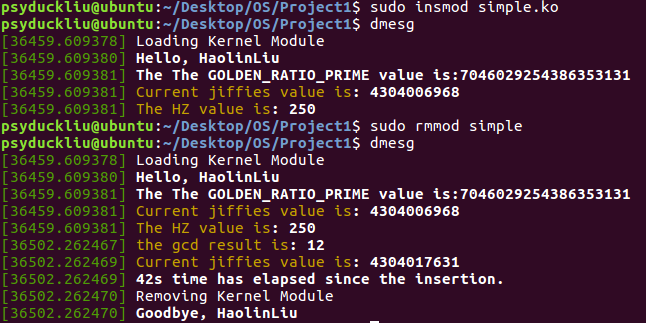
\includegraphics[width=0.7\linewidth]{pic1}
		\caption[simple.c]{simple.c}
		\label{fig:pic1}
	\end{figure}
	\subsection{Part 2-assignment 1}
	\begin{figure}[h]
		\centering
		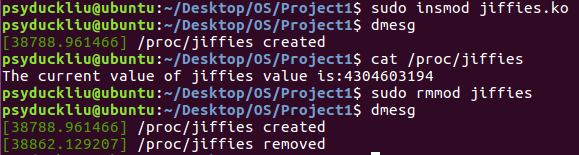
\includegraphics[width=0.7\linewidth]{pic2}
		\caption[jiffies.c]{jiffies.c}
		\label{fig:pic2}
	\end{figure}
	\subsection{Part 3-assignment 2}
	\begin{figure}[h]
		\centering
		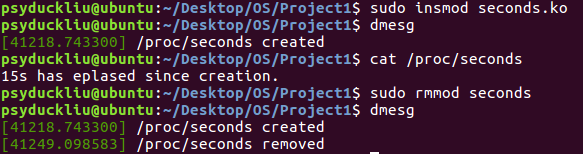
\includegraphics[width=0.7\linewidth]{pic3}
		\caption[seconds.c]{seconds.c}
		\label{fig:pic3}
	\end{figure}
	
	
	
	
	
	
	
	
	
\end{document}